% ==============================================================================
% Section 4: ZwerGe-UI
% ==============================================================================

\section{\textsc{ZwerGe-UI}}
\label{sec:method}

\begin{figure*}[t]
\centering
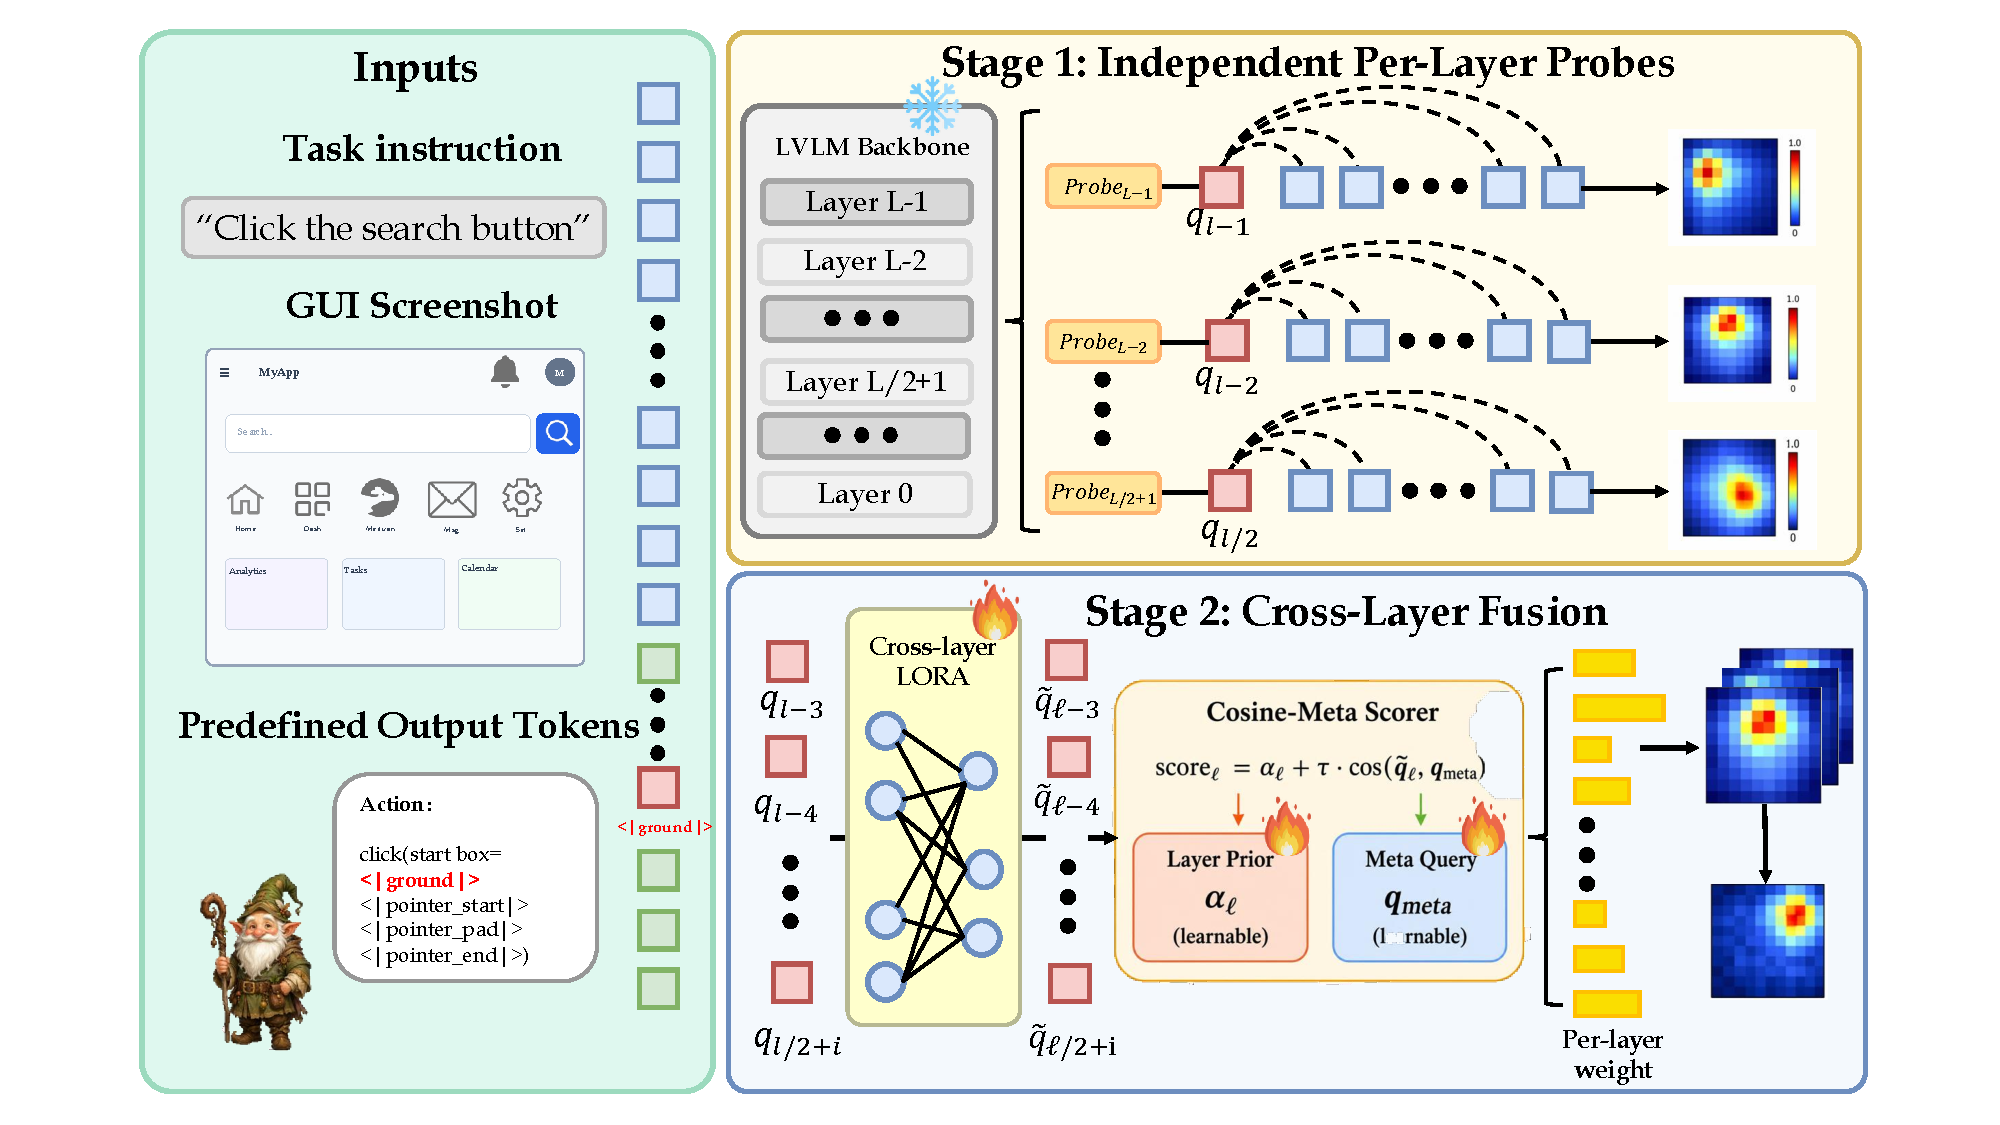
\includegraphics[width=0.95\textwidth]{figs/pipeline.pdf}
\caption{\textbf{Overview of \textsc{ZwerGe-UI}.} A frozen backbone exposes layerwise hidden states from a single prefill; independent probes decode intermediate-layer spatial posteriors, a cross-layer fusion head selects the reliable depth per sample, and a training-free confidence gate routes each sample between the fused point and the native autoregressive coordinate.}
\label{fig:zwerge_pipeline}
\end{figure*}

The per-layer probes of \S\ref{sec:probe} are independent, and the best layer varies by sample (\S\ref{sec:analysis}, Finding~1). We add two lightweight components on top of the frozen probes, shown in Figure~\ref{fig:zwerge_pipeline}: a cross-layer fusion head that selects the reliable depth per sample, and a training-free confidence gate that decides when to trust the fused point over the backbone's own decoder. Both reuse the single prefill of \S\ref{sec:probe}, so the retrofit adds negligible compute over the native baseline.

% ------------------------------------------------------------------------------
\subsection{Cross-Layer Fusion}
\label{sec:method:stage2}
% ------------------------------------------------------------------------------

We draw active layers $\mathcal{L}_{\mathrm{active}}\subset\mathcal{L}_{\mathrm{probe}}$ from the spatial plateau identified in \S\ref{sec:analysis} and fuse their posteriors. A cross-layer LoRA refines each anchor query $\mathbf{h}^{(\ell)}_{t^*}$ into $\tilde{\mathbf{q}}_\ell$; a cosine-meta scorer then assigns per-layer weights:
\begin{equation}
  \omega_\ell = \mathrm{softmax}\!\left(\alpha_\ell + \tau^{-1}\cos\!\big(\tilde{\mathbf{q}}_\ell,\,\mathbf{q}_{\mathrm{meta}}\big)\right),\qquad
  p_{\mathrm{final}} = \sum_{\ell\in\mathcal{L}_{\mathrm{active}}}\omega_\ell\,p_\ell,
  \label{eq:fusion}
\end{equation}
where $\alpha_\ell$ is a sample-independent trainable prior on layer $\ell$'s average quality, $\mathbf{q}_{\mathrm{meta}}$ is a global trainable meta-query serving as a soft prototype of the ideal grounding representation, and $\tau$ is a learnable temperature. Layers whose refined query aligns with $\mathbf{q}_{\mathrm{meta}}$ receive higher weight for the current input. The LoRA contributes ${\approx}200$K parameters, two orders of magnitude below a single probe.

Stage~2 loads the Stage-1 probes; the backbone and inactive probes stay frozen, while the fusion head and the active probes remain trainable, with loss
\begin{equation}
  \mathcal{L}_{\mathrm{S2}} = D_{\mathrm{KL}}(\mathbf{y}\,\|\,p_{\mathrm{final}}) + \tfrac{\lambda}{|\mathcal{L}_{\mathrm{active}}|}\sum_\ell D_{\mathrm{KL}}(\mathbf{y}\,\|\,p_\ell),\quad \lambda=0.2,
  \label{eq:loss_s2}
\end{equation}
so the per-layer auxiliary term gives every active probe a direct gradient signal and no single layer is neglected.

% ------------------------------------------------------------------------------
\subsection{Training-Free Gated Decoding}
\label{sec:method:ensemble}
% ------------------------------------------------------------------------------

The fusion posterior $p_{\mathrm{final}}$ is patch-level, not a coordinate. In one prefill we read both the fused point $\mathbf{f}$, produced by a training-free posterior-to-point decoder detailed in the supplementary material, and the backbone's native autoregressive coordinate $\mathbf{n}$, and route between them with a GT-free gate on the posterior sharpness: emit $\mathbf{f}$ when the margin $m=p_{\mathrm{final}}^{(1)}-p_{\mathrm{final}}^{(2)}$, the difference between the top-two single-patch probabilities, exceeds $\tau$, otherwise emit $\mathbf{n}$. A sharp mode means the probe is confident in one location; a diffuse mode means the native serializer should be trusted. The default is $\tau{=}0.25$, while the main results use $0.20$. This instantiates the paper's thesis: the intermediate layer identifies \emph{where} the target is, and a confidence gate decides when to trust that signal over the final-layer serializer.

\paragraph{Fairness and cost.}
The comparison against the native baseline is protocol-symmetric: both points are evaluated under the same strict point-in-box metric on the same cached run, and the gate uses no labels. The ensemble adds no autoregressive generation over the baseline. The native generate is the baseline's own computation, and the fused point reads intermediate activations that the backbone already produces in that same forward; in principle the two share one prefill, so the full retrofit is realizable at the cost of a single forward pass.
